% class
\documentclass[a4paper,12pt,xelatex,ja=standard]{bxjsarticle}

% packages
%% mathematical notations
\usepackage{amsthm,amsmath,amssymb,amsfonts} % mathematical notations
\usepackage{bm} % bold character
\usepackage{latexsym} % more mathematical notations
\usepackage{physics} % physical notations
%% graphs
\usepackage{graphicx, xcolor} % graph
\usepackage{circuitikz} % for circuit elements
\usepackage{float} % positioning of graphs
\usepackage{siunitx} % SI units
\usepackage{tikz} % graphic elements
\usepackage{wrapfig} % must be after float package.
\usepackage{askmaps} % Karnaugh map
%% type system
\usepackage{bussproofs} % proof tree
%% code
\usepackage[ruled,vlined]{algorithm2e} % pseudo code
\usepackage{listings} % source code
\usepackage{inconsolata}
\lstset{
  basicstyle=\footnotesize,
  numbers=left,
  frame={tb}
}
\usetikzlibrary{automata, positioning}
\tikzset{
  ->,
  >={Stealth[round]},
  auto,
  every state/.style={draw}
}

% Basic information
\title{電子情報学専攻 \, 専門 \\ 平成27年 \, 解答・解説}
\author{diohabara}
\date{\today}

\begin{document}
\maketitle

\section*{第1問\ 電気・電子回路}

\section*{第2問\ 計算機アーキテクチャ}
\subsection*{(1)}
\begin{itemize}
  \item $\alpha$: r1
  \item $\beta$: -1
  \item $\gamma$: r1
  \item $\delta$: r4
\end{itemize}

\subsection*{(2)}
\begin{itemize}
  \item (i): b
  \item (ii): a
\end{itemize}

\subsection*{(3)}
求める動作周波数は
\[
  \frac{1}{(250 + 100 + 150 + 100 + 300 + 150) \cdot 10^{-12}} = \frac{10^{12}}{1050}\text{[clock/s]}
\]

\subsection*{(4)}
\begin{itemize}
  \item I1, I2: 構造ハザード
  \item (I1, I2): データハザード
  \item (I4, I5): 制御ハザード
\end{itemize}

\subsection*{(5)}
TODO

\subsection*{(6)}
TODO

\section*{第3問\ アルゴリズムとデータ構造}
\subsection*{(1)}
各ステップにおいて、$B$に含まれる頂点と$V \setminus B$に含まれる頂点を結ぶ辺のうち重みが最小である辺$e = \{u, v\} (u \in V \setminus B, v \in B)$が最小全域木に含まれることを示す。\\
連結グラフなら最小全域木が必ず存在し、このうちの1つを$T \subseteq E$とする。$T$が$e$を含むならok。
含まない場合は、$B$と$V \setminus B$を結ぶある辺$f = e$存在し、$(f\text{の重み}) \geq (e\text{の重み})$が成立する。
この最小全域木には$u, v$をつなぐパス($f$を含む)が存在するので、$T$に$e$を追加すると閉路ができ、そこから$f$を取り除いた辺集合は全域木であることが言える。
重みの総和は$T$の重みの総和以下であるのでこれもまた最小全域木である。

\subsection*{(2)}
最小全域木は以下の通り。
\begin{figure}[H]
  \centering
  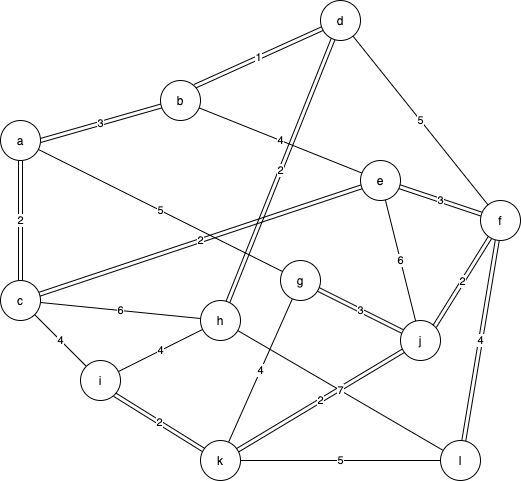
\includegraphics[width=11cm]{images/2016_min_spanning_tree.png}
\end{figure}

\subsection*{(3)}
\begin{lstlisting}[language=Python, caption=プリム法]
def primMST():
    T = set()
    for i in range(1, n):
        edge = set()
        min_cost = inf
        for v in (V - B):
            u = nearest[v]
            if mindist[v] == -1:
                continue
            if L[u, v] < min_cost:
                min_cost = L[u, v]
                edge = {u, v}
        T.append(edge)

\end{lstlisting}

\subsection*{(4)}
$O(|V|^2)$\\
nearestとmindistの更新を素朴にやると$O(|V|^2)$なので、全体で$O(|V|^3)$だが、$V \setminus B$に含まれる各頂点までの最小コストを記録しておいて、各ステップにおいてその最小コストが最小の頂点を$V$に加えるようにすれば$O(|V|^2)$に計算量をできる。

\subsection*{(5)}
二分ヒープとは二分木を使って実装されるヒープのことである。
ヒープとは各ノードはその子ノードよりも大きいか等しい。また、平衡二分木となっている。

\subsection*{(6)}
\subsubsection*{適用の仕方}
二分ヒープheapに$B$に含まれる頂点から伸びている辺を入れて重みが小さい順に取り出すことにする。\\
各ステップにおいて
\begin{enumerate}
  \item heapから辺を1つ取り出す
  \item その辺の両端点がそれぞれ$B$と$V \setminus B$に含まれていればその辺を採用して新たに$V$に加わった頂点から伸びている辺をすべてheapに追加する。そうでなければその辺は削除して1に戻る
\end{enumerate}
という処理を行う。

\subsubsection*{計算量}
heapへの追加・削除はそれぞれ$O(\log |E|)$でできて、各頂点から伸びる辺の探索は$O(|V|)$なので全体で$O(|V|^2 \log |E|)$。
これでは(4)で見積もった計算量より悪い。しかし、グラフを隣接リストで実装すると全体で$O((|V| + |E|) \log |E|) = O(|E| \log |E|)$となる。

\subsubsection*{頂点の数$n$と辺の数$m$の関係}
完全グラフのような辺の数$m$が頂点の数$n$の事情のオーダーの場合は計算量が悪化するが、そこまで辺が大きくなければ効率化できる。

\section*{第4問\ 情報理論}
\subsection*{(1)}
$x_5 = x_1 \oplus x_2 \oplus x_3 \oplus x_4$とすればよい。
$x_1, \dots, x_4$のどれか1つが反転した際に$x_5$は1となり検出ができる。

\subsection*{(2)}
情報ビットの1の個数が奇数のとき、検査ビットは1となる。よって、情報ビットの1の個数が最小の1のとき検査ビットは1となり$(0, 0, 0, 0, 0)$とのハミング距離は2となる。\\
情報ビットの1の個数が偶数のとき、検査ビットは0となる。よって、情報ビットの1の個数が0を除いて最小の2のとき検査ビットは0となり$(0, 0, 0, 0, 0)$とのハミング距離は2となる。\\
よって最小ハミング距離は2であり、その符号語の1つに$(1, 1, 0, 0, 0)$が挙げられる。

\subsection*{(3)}
すべての符号語を表にすると以下の通り。
\begin{table}[H]
  \centering
  \begin{tabular}{|l|l|l|l|l|l|l|}
  \hline
  $x_1$ & $x_2$ & $x_3$ & $x_4$ & $x_5$ & $x_6$ & $x_7$ \\ \hline \hline
  0     & 0     & 0     & 0     & 0     & 0     & 0     \\ \hline
  0     & 0     & 0     & 1     & 1     & 1     & 0     \\ \hline
  0     & 0     & 1     & 0     & 0     & 1     & 1     \\ \hline
  0     & 0     & 1     & 1     & 1     & 0     & 1     \\ \hline
  0     & 1     & 0     & 0     & 1     & 1     & 1     \\ \hline
  0     & 1     & 0     & 1     & 0     & 0     & 1     \\ \hline
  0     & 1     & 1     & 0     & 1     & 0     & 0     \\ \hline
  0     & 1     & 1     & 1     & 0     & 1     & 0     \\ \hline
  1     & 0     & 0     & 0     & 1     & 0     & 1     \\ \hline
  1     & 0     & 0     & 1     & 0     & 1     & 1     \\ \hline
  1     & 0     & 1     & 0     & 1     & 1     & 0     \\ \hline
  1     & 0     & 1     & 1     & 0     & 0     & 0     \\ \hline
  1     & 1     & 0     & 0     & 0     & 1     & 0     \\ \hline
  1     & 1     & 0     & 1     & 1     & 0     & 0     \\ \hline
  1     & 1     & 1     & 0     & 0     & 0     & 1     \\ \hline
  1     & 1     & 1     & 1     & 1     & 1     & 1     \\ \hline
  \end{tabular}
\end{table}

\subsection*{(4)}
表で1の個数が最小のものを探せば良く、3。

\subsection*{(5)}
最小ハミング距離$d_H$に対して$2d + 1 \leq d_H$となる最大の整数$d$を考える。このとき、$d$ビットの誤り訂正が可能。
\begin{itemize}
  \item (1)の場合、最小ハミング距離は2なので$d=0$となる。すなわち誤り訂正はできない
  \item (3)の場合、最小ハミング距離は3なので$d=1$となる。したがって、1ビットの誤りまでなら誤り訂正が可能。
\end{itemize}

\subsection*{(6)}
\subsubsection*{対応手法}
短い区間に多数の誤りが集中するバースト誤りに対して、符号の順序を入れ替え、同じブロックのデータを分散させ、ある区間に誤りが集中しないようにする。

\subsubsection*{利害得失}
バースト誤りの訂正が可能になるという利点がある。一方で伝送速度が犠牲になるという欠点がある。

\section*{第5問\ 信号処理}
\subsection*{(1)}
\subsubsection*{フーリエ変換の定義}
\[
  F(\omega) = \int^{\infty}_{-\infty}f(t)e^{-j \omega t}dt
\]

\subsubsection*{フーリエ変換とフーリエ級数展開の違い}
フーリエ変換は時間軸上で連続かつ非周期的な信号を扱うのに対して、フーリエ級数展開は時間軸上で連続かつ周期的な信号を扱う。そのため$\omega$は基本周波数の整数倍しか取らず、周波数領域について離散的になる。\\
また、フーリエ級数展開は信号全体を扱わず、1周期だけを切り出して複素正弦はの足し合わせで表せる点でもフーリエ変換と異なっている。

\subsection*{(2)}
$|F(\omega)|$は信号を複素正弦波$e^{j \omega t}$を基底として分解したときの$\omega$成分の振幅を表している。したがって、振幅の2乗$|F(\omega)|^2$はパワーに対応する。\\
また、基底となる関数の直交性より角周波数$\omega$成分のパワーは他の成分の影響を受けないため$|F(\omega)|^2$と$\omega$成分のパワーは1対1に対応している。

\subsection*{(3)}
パーセバルの等式を証明する。\\
2つの関数$f(x)$と$g(x)$の畳み込み積分の式は次の通り。

\[
  h(x) = \int^{\infty}_{- \infty}f(t)g(x - t) dt
\]

これは任意の$x$において成り立つので、ここに$x = 0$を代入する。以下の式が得られる。

\begin{equation}
  \begin{split}
    \label{eq52:1}
    \int^{\infty}_{- \infty}f(t)g(-t) dt = k' \int^{\infty}_{- \infty}F(\omega) G(\omega) d \omega \\
    \int^{\infty}_{- \infty}f(-t)g(t) dt = k' \int^{\infty}_{- \infty}F(\omega) G(\omega) d \omega
  \end{split}
\end{equation}

$g(t) = \overline{f(-t)}$とすれば左辺は$|f(t)|^2$に一致する。このとき、以下の式が成り立つ。

\begin{equation}
  \begin{split}
    G(\omega)
      &= \int^{\infty}_{- \infty} g(t) e^{j \omega t} dt \\
      &= \int^{\infty}_{- \infty} \overline{f(-t)} e^{j \omega t} dt \\
  \end{split}
\end{equation}

両辺の複素共役を取ると

\begin{equation}
  \begin{split}
    \label{eq52:2}
    \overline{G(\omega)}
      &= \int^{\infty}_{- \infty} f(-t) e^{j \omega t} dt \\
      &= \int^{\infty}_{- \infty} f(\tau) e^{-j \omega \tau} d\tau \\
      &= F(\omega)
  \end{split}
\end{equation}

(\ref{eq52:1})に(\ref{eq52:2})を代入すると等式が成り立つことが示された。また、このときの比例定数$k$は$k'$に一致する。

\subsection*{(4)}

パーセバルの等式は左辺の時間領域のエネルギーと右辺の周波数領域のエネルギーが定数倍を除いて等しいことを意味する。

\end{document}
